% !TeX document-id = {0be8c18c-9430-4e9a-bdd9-12beadebfebc}
% !TeX TXS-program:bibliography = txs:///biber
\documentclass[11pt]{beamer}

\usepackage[brazilian]{babel}

\uselanguage{portuguese}
\languagepath{portuguese}
\deftranslation[to=portuguese]{Theorem}{Teorema}
\deftranslation[to=portuguese]{theorem}{teorema}
\deftranslation[to=portuguese]{Example}{Exemplo}
\deftranslation[to=portuguese]{example}{exemplo}
\deftranslation[to=portuguese]{Lemma}{Lema}
\deftranslation[to=portuguese]{lemma}{Lema}
\deftranslation[to=portuguese]{Corollary}{Corolário}
\deftranslation[to=portuguese]{corollary}{corolário}
%\deftranslation[to=portuguese]{and}{e}


\usepackage[utf8]{inputenc}
\usepackage[T1]{fontenc}
\usepackage{lmodern}
\usepackage{amsmath}
\usepackage{amssymb}
\usepackage{mathtools}
\usepackage{color}
\usepackage{pgfplots}
\usepackage{tikz}
\usepackage{subcaption}
%\usepackage{appendixnumberbeamer}

\newenvironment{transitionframe}{
	\setbeamercolor{background canvas}{bg=yellow}
	\begin{frame}}{
	\end{frame}
}
\usetheme{default}
\usefonttheme{structuresmallcapsserif}

%% I use a beige off white for my background
\definecolor{MyBackground}{RGB}{255,253,218}
\useinnertheme[shadow]{rounded}
\setbeamercolor{block title}{bg=MyBackground}
\setbeamercolor{block body}{bg=MyBackground}
\setbeamercolor{example title}{bg=MyBackground}
\setbeamercolor{example body}{bg=MyBackground}


\newcommand{\blue}[1]{\textcolor{blue}{#1}}
\newcommand{\red}[1]{\textcolor{red}{#1}}
\newcommand{\purple}[1]{\textcolor{purple}{#1}}
\newcommand{\gray}[1]{\textcolor{gray}{#1}}
\setbeamertemplate{navigation symbols}{}
%\setbeamertemplate{page number in head/foot}[appendixframenumber]

%\usepackage{graphics}
\usepackage{graphicx}

\definecolor{blue_emph}{RGB}{0,114,178}
\definecolor{red}{RGB}{213,94,0}
\definecolor{yellow}{RGB}{240,228,66}
\definecolor{green}{RGB}{0,158,115}
\definecolor{purple}{RGB}{204,121,167}
\definecolor{orange}{RGB}{230,159,0}
\definecolor{lightblue}{RGB}{86,180,233}

%\setbeamercolor{frametitle}{fg=blue}
%\setbeamercolor{title}{fg=blue}
\setbeamertemplate{footline}[frame number]
\setbeamertemplate{navigation symbols}{} 
\setbeamertemplate{itemize items}{-}
%\setbeamercolor{itemize item}{fg=blue}
%\setbeamercolor{itemize subitem}{fg=blue}
\setbeamertemplate{enumerate items}[default]
%\setbeamercolor{enumerate subitem}{fg=blue}
\setbeamercolor{button}{bg=MyBackground,fg=blue}
\usefonttheme{structuresmallcapsserif}

%\setbeamercolor{section in toc}{fg=blue}
%\setbeamercolor{subsection in toc}{fg=red}
\setbeamersize{text margin left=1em,text margin right=1em} 


\usepackage{appendixnumberbeamer}
\usepackage{pdfpages}
\usepackage[
backend=biber,
uniquename=false,
uniquelist=false,
style=authoryear,
natbib=true
]{biblatex}
\addbibresource{../bibliography.bib}

\newenvironment{wideitemize}{\itemize\addtolength{\itemsep}{10pt}}{\enditemize}
\newenvironment{wideenumerate}{\enumerate\addtolength{\itemsep}{10pt}}{\endenumerate}
\newenvironment{halfwideitemize}{\itemize\addtolength{\itemsep}{0.5em}}{\enditemize}
\newenvironment{halfwideenumerate}{\enumerate\addtolength{\itemsep}{0.5em}}{\endenumerate}


\author{Luis A. F. Alvarez}
\title{EAE1223: Econometria III}
\subtitle{Aula 9 - Modelos vetoriais autorregressivos estruturais}
%\logo{}
%\institute{}
\date{\today}
%\subject{}
%\setbeamercovered{transparent}

\def\signed #1{{\leavevmode\unskip\nobreak\hfil\penalty50\hskip2em
		\hbox{}\nobreak\hfil(#1)%
		\parfillskip=0pt \finalhyphendemerits=0 \endgraf}}

\newsavebox\mybox
\newenvironment{aquote}[1]
{\savebox\mybox{#1}\begin{quote}}
	{\signed{\usebox\mybox}\end{quote}}

\begin{document}

\begin{frame}[plain]
	\maketitle
\end{frame}

\begin{frame}{Um modelo para a descrição de uma economia}
	\begin{itemize}
		\item 	Seja $\{ \boldsymbol{Y}_t\}_{t\in \mathbb{Z}}$ um processo vetorial de interesse, onde $\boldsymbol{Y}_t$ consiste de $d$ variáveis econômicas, sobre as quais a teoria econômica têm algo a nos dizer sobre o comportamento conjunto.
		\item Um {\color{blue}modelo estrutural (causal) linear} para estas variáveis consiste em um sistema de $d$ equações da forma:
		\begin{equation} \label{eq_struct}
			\boldsymbol{A}_0 \boldsymbol{Y}_t = \boldsymbol{a} + \sum_{j=1}^p\boldsymbol{A}_j \boldsymbol{Y}_{t-j} + \boldsymbol{\epsilon}_t\, ,
		\end{equation}
		onde $\boldsymbol{A}_0$ é uma matriz $d \times d$ que explicita as relações contemporâneas (causais) entre as variáveis, e $\boldsymbol{\epsilon}_t$ é um ruído branco {\color{blue}contemporaneamente não correlacionado}, isto é $$ \mathbb{V}[\boldsymbol{\epsilon}_t] = \begin{bmatrix}
			\sigma_{1}^2 & 0 & \ldots & 0 \\
			0 & \sigma^2_2 & \ldots & 0 \\
			\vdots & \ldots & \ddots & \vdots \\
			0 & 0 & \ldots & \sigma^2_d
		\end{bmatrix}= \Omega_\epsilon $$
		\end{itemize}


\end{frame}

\begin{frame}{Choques econômicos fundamentais }
	\begin{itemize}
		\item A hipótese de que os erros de cada uma das equações são contemporaneamente não correlacionados supõe que o modelo que descreve a economia esteja {\color{blue}bem especificado}, de modo que o choque da $j$-ésima equação reflete a incerteza econômica fundamental associada a $Y_{jt}$.
		\begin{itemize}
			\item $\epsilon_{jt}$ reflete choques (surpresas ou inovações, não antecipadas com base no passado) nos determinantes essenciais de $Y_{jt}$, e não nos determinantes indiretos (via outras variáveis do sistema) de $Y_{jt}$. 
	
		\end{itemize}
				\item Esse tipo de hipótese é presumida em uma das perguntas clássicas da macroeconomia: quanto da flutuação econômica pode ser atribuída à política monetária vs fatores reais?
				\begin{itemize}
					\item Pergunta presume que existem inovações fundamentais, contemporaneamente ortogonais (não correlacionadas), em fatores monetários e reais, que permitem pensar nesta decomposição, visto que ela não faz sentido se os fatores fundamentais não fossem fundamentais (i.e. correlacionados).
					\item Veremos como nossa metodologia permite fazer explicitamente esta decomposição.
				\end{itemize}
	
	\end{itemize}
\end{frame}

\begin{frame}{Exemplo}
	\begin{itemize}
			\item Considere o comportamento conjunto de inflação ($\pi_t$), desemprego ($u_t$), expectativas de inflação ($\pi^e_t$) e taxa de juros nominal ($i_t$):
	\end{itemize}
			\begin{align}
		\pi_t = \sum_{j={\color{blue}1}}^p \theta_j \pi_{t-j} + \sum_{j={\color{red}0}}^p \beta_j (u_{t-j}-\bar{u}_{\text{neutro}}) + \sum_{j={\color{red}0}}^p \gamma_j \pi_{t-j}^e + \epsilon_{\pi,t} \tag{CP} \\
		u_t - \bar{u} = \sum_{j={\color{blue}1}}^p \omega_j (u_{t-j}-\bar{u}) + \sum_{j={\color{red}0}}^p \alpha_j (i_{t-j} - \pi^e_{t-j})  + \epsilon_{u,t} \tag{IS} \\  i_t = \bar{i} + \sum_{j={\color{blue}1}}^p \psi_j i_{t-j} + \sum_{j={\color{red}0}}^p \kappa_j (\pi_{t-j}-\pi_{\text{M}}) + \sum_{j={\color{red}0}}^p \phi_j (\pi_{t-j}^e-\pi_{\text{M}}) + \epsilon_{i,t}\tag{RM}\\
		\pi^e_t = \mu \pi_{M} +  \sum_{j={\color{blue}1}}^p \iota_j \pi^e_{t-j} + \theta_3 \sum_{j={\color{red}0}}^p (\nu_{1j} \pi_{t-j} + \nu_{2j} u_{t-j} + \nu_{3j} i_{t-j}) + \epsilon_{e,t} \tag{FE}
	\end{align}
	onde $\epsilon_{\pi,t}$ são choques de oferta (CP), $\epsilon_{u,t}$ choques de demanda (IS), $\epsilon_{i,t}$ são surpresas de política monetária (RM), e $\epsilon_{e,t}$ são ruídos na formação de expectativas.

\end{frame}

\begin{frame}{Representação autorregressiva do modelo linear estrutural}
	\begin{itemize}
		\item Se o sistema \eqref{eq_struct} oferece uma descrição {\color{blue}completa} da evolução de $\boldsymbol{Y}_t$, então, para uma dada trajetória pretérita $\{\boldsymbol{Y}_s: s \leq t-1\}$, e valores dos choques fundamentais $\boldsymbol{\epsilon}_t$, existe um único valor de $\boldsymbol{Y}_t$  que satisfaz \eqref{eq_struct}.
		\item Nesse caso, a matriz $\boldsymbol{A}_0$ admite inversa $\boldsymbol{B}= \boldsymbol{A}_0^{-1}$, e o sistema admite {\color{blue}representação autorregressiva}:
		
		\begin{equation}
			\label{eq_arriv}
			\boldsymbol{Y}_t = \underbrace{\boldsymbol{c}}_{= \boldsymbol{B}\boldsymbol{a}} + \sum_{j=1}^p \underbrace{\boldsymbol{C}_j}_{=\boldsymbol{B} \boldsymbol{A}_j} \boldsymbol{Y}_{t-j}  + \boldsymbol{B}\boldsymbol{\epsilon}_t\, .
		\end{equation}
		
		\item Modelo VAR em que o ruído branco $\boldsymbol{B}\boldsymbol{\epsilon}_t$ é uma combinação linear de choques fundamentais.
		\item Matriz $\boldsymbol{B}$ incorpora o efeito contemporâneo de inovações fundamentais sobre as variáveis em $\boldsymbol{Y}_t$. 
	\end{itemize}
\end{frame}

\begin{frame}{Modelo SVAR(p)}
\begin{itemize}
	\item 	Em diversas situações, não necessariamente queremos partir de \eqref{eq_struct} para chegar a \eqref{eq_arriv}
	\begin{itemize}
		\item Não necessariamente temos uma descrição completa da economia.
		\item De modo relacionado, a formulação \eqref{eq_arriv} pode ser compatível com mais de uma formulação estrutural linear completa.
	\end{itemize}
	\item Nesses casos, podemos definir diretamente {\color{blue}um modelo vetorial autorregressivo (semi)estrutural de ordem $p$}, SVAR(p), como o processo
	
		\begin{equation}
		\label{eq_svar}
		\boldsymbol{Y}_t = \boldsymbol{c}+ \sum_{j=1}^p \boldsymbol{C}_j \boldsymbol{Y}_{t-j} + \boldsymbol{B}\boldsymbol{\epsilon}_t\, ,
	\end{equation}
	onde $\boldsymbol{\epsilon}_t$ são inovações fundamentais, isto é ruídos brancos não contemporaneamente correlacionados, e $\boldsymbol{B}$ é a matriz que captura os efeitos contemporâneos das inovações fundamentais sobre $\boldsymbol{Y}_t$.
\end{itemize}
\end{frame}

\begin{frame}{Função de resposta ao impulso}
	\begin{itemize}
		\item Os efeitos causais dinâmicos, na modelagem SVAR, são capturados pelos efeitos de surpresas dos choques fundamentais sobre o comportamento do sistema.
		\begin{itemize}
			\item Note que, por construção, $\boldsymbol{\epsilon}_t$ captura fatores não antecipados com base no passado. 
			\item Como $\boldsymbol{\epsilon}_t$ é não contemporaneamente correlacionado, faz sentido pensar em surpresas em um de seus componentes, mantidos os outros constantes.
	\end{itemize}
	\item Formalmente, o efeito causal de uma surpresa de uma unidade na $j$-ésima inovação do sistema em $t$, $\epsilon_{jt}$, sobre a $i$-ésima variável do sistema em $t+h$, $h\geq 0$, é dada pela {\color{blue}função de resposta ao impulso}
	$$F_{h}(i|j)  = \frac{\partial Y_{i,t+h}}{\partial \epsilon_{j,t}}$$
	\item  $F_{0}(i|j) = \boldsymbol{B}_{ij}$, $F_{1}(i|j) = \sum_{l=1}^d\boldsymbol{C}_{1, i,l} \boldsymbol{B}_{lj} = \sum_{l=1}^d\boldsymbol{C}_{1, i,l} F_{0}(l|j)$, $F_2(i|j) = \sum_{l=1}^d \boldsymbol{C}_{1, i,l} F_{1}(i|j) + \sum_{l=1}^d\boldsymbol{C}_{2, i,l} F_{0}(i|j)$, etc.
	\end{itemize}
\end{frame}

\begin{frame}{FRI normalizada, FRI acumulada}
\begin{itemize}
	\item Em diversos casos, é costumeiro normalizar a FRI pelo desvio padrão dos choques, isto é, reporta-se:
	$$F_h(i|j){\color{red}\times} \sigma_{j,t}\,.$$
	
	\begin{itemize}
		\item 	Neste caso, os coeficientes são interpretáveis como o efeito causal de uma surpresa de um desvio padrão na $j$-ésima inovação.
	\end{itemize}
	\item Também podemos reportar a FRI acumulada:
	
	$$\sum_{\tau=0}^h F_\tau(i|j)\, .$$
	
	\begin{itemize}
		\item Se a $i$-ésima variável está em primeiras diferenças, a FRI acumulada reporta o efeito da surpresa sobre o nível da série em $t+h$.
		\item Alternativamente, FRI acumulada pode ser interpretada como o efeito de uma sequência de surpresas (por construção, não antecipadas) de uma unidade na $j$-ésima variável do sistema por $h$ períodos.
		\begin{itemize}
			\item Note que, pela crítica de Lucas, sabemos que isto é \textbf{diferente} do efeito de um aumento permanente de uma unidade sobre a $j$-ésima variável do sistema.
		\end{itemize}
	\end{itemize}
	
\end{itemize}
\end{frame}


\begin{frame}{Decomposição da variância do erro de predição}
		\begin{itemize}
		\item Com base no SVAR(p), somos capazes, analogamente ao VAR(p), de calcular previsões para $T+h$, com dados até $T$, $\boldsymbol{Y}_{T+h|T}$:
		\begin{align*}
			\boldsymbol{Y}_{T+1|T} = \boldsymbol{c} + \sum_{j=0}^{p-1} \boldsymbol{C}_{j+1} \boldsymbol{Y}_{T-j} \\
				\boldsymbol{Y}_{T+2|T} = \boldsymbol{c} +  {\color{red}\boldsymbol{C}_{j}\boldsymbol{Y}_{T+1|T}} +  \sum_{j=0}^{p-2} \boldsymbol{C}_{j+2} \boldsymbol{Y}_{T-j}  \\
				\vdots
		\end{align*}
	\end{itemize}
	\begin{itemize}
\item O erro de previsão no horizonte $h$ é dado por $\boldsymbol{Y}_{T+h} - \boldsymbol{Y}_{T+h|T}$.
\item Dada a natureza estrutural dos choques, é possível mostrar que somos capazes de decompor aditivamente a {\color{blue}variância do erro de previsão de cada variável} na contribuição de cada choque:
$$\mathbb{V}[\boldsymbol{Y}_{i,T+h} - \boldsymbol{Y}_{i, T+h|T}] = \sum_{j=1}^d \text{contribuição do choque j}$$
	\end{itemize}
\end{frame}

\begin{frame}{Decomposição da variância do erro de predição (cont.)}
	\begin{halfwideitemize}

		\item Decomposição da variância do erro de predição nos permite dizer, para cada horizonte, quantos \% da incerteza futura depende de cada uma das inovações estruturais.
				\item Fácil de ver que a decomposição não depende de $t$, mas tão somente do horizonte e variável de interesse,
		\item Se tomamos $h \to \infty$, temos uma decomposição da variância de longo prazo (incondicional) do sistema.
		\begin{itemize}
			\item Por exemplo, podemos dizer quanto da variabilidade da atividade econômica se deve a choques monetários.
		\end{itemize}
	\end{halfwideitemize}
\end{frame}


\begin{frame}{SVAR(p) e VAR(p)}
\begin{itemize}
	\item Note que um SVAR(p) da forma \eqref{eq_svar} sempre define um VAR(p).
	\item De fato, se definimimos $\boldsymbol{u}_t = \boldsymbol{B}\boldsymbol{\epsilon}_t$,  podemos escrever:
	\begin{equation}
		\label{eq_rvar}
		\boldsymbol{Y}_t = \boldsymbol{c}+ \sum_{j=1}^p \boldsymbol{C}_j \boldsymbol{Y}_{t-j} + \boldsymbol{u}_t\, ,
	\end{equation}
	onde $\boldsymbol{u}_t$ é um {\color{blue}ruído branco contemporaneamente correlacionado}, cuja matriz de variância é dada por $\mathbb{V}[\boldsymbol{u}_t] = \boldsymbol{B}\mathbb{V}[\boldsymbol{\epsilon}_t] \boldsymbol{B}' =\Sigma$.
	\begin{itemize}
		\item VAR(p) em que ruído branco segue da combinação linear de choques estruturais.
		\item Essas combinações lineares produzem um ruído branco contemporaneamente correlacionado, na medida em que choques fundamentais afetam simultaneamente mais de uma variável do sistema.
	\end{itemize}
	\item A um VAR(p) derivado de um SVAR(p), daremos o nome de {\color{blue}modelo vetorial em forma reduzida}.
\end{itemize}
\end{frame}

\begin{frame}{O problema de identificação causal no SVAR(p)}
\begin{itemize}
	\item Recorde-se que, sob condições bastantes gerais, podemos estimar consistentemente os parâmetros de um VAR(p).
	\begin{itemize}
		\item Resultado vale para séries estacionárias, e mesmo para processos integrados (embora, nesse caso, a inferência com base em distribuições convencionais não seja válida).
	\end{itemize}
	\item Como os parâmetros do VAR(p) são consistentemente estimáveis, segue que, com $T$ grande, somos capazes de recuperar aproximadamente as {\color{blue}inovações reduzidas} $\{\boldsymbol{u}_t : 1 \leq t \leq T\}$. 
	\begin{itemize}
		\item Como essas inovações são recuperáveis com $T$ grande, também somos capazes de estimar consistentemente $\Sigma = \mathbb{V}[\boldsymbol{u}_t]$.
	\end{itemize}
	\item O {\color{blue}problema de identificação causal no SVAR(p)} consiste em prover condições a partir das quais sejamos capazes de {\color{blue}recuperar os choques estruturais $\boldsymbol{\epsilon}_t$ a partir da observação de $\boldsymbol{u}_t$}.
	\begin{itemize}
		\item Ideia é encontrar condições que nos permitam descorrelacionar os choques reduzidos em termos das inovações fundamentais.
	\end{itemize}
\end{itemize}
\end{frame}

\begin{frame}{Identificação dos choques estruturais}
	\begin{itemize}
		\item Para descorrelacionar $\boldsymbol{u}_t$, precisamos recuperar a matriz $\boldsymbol{B}$.
		\item Em geral, as análises estruturais preferem ser agnósticas sobre os componentes autorregressivos do processo $\implies$ coeficientes $\boldsymbol{C}_j$ não nos trazem informação sobre $\boldsymbol{B}$.
		\begin{itemize}
			\item Componentes autorregressivos aparecem pois queremos ser relativamente agnósticos sobre a ``propagação'' de choques intertemporalmente (teoria dificilmente nos diz algo sobre isso), o que sugere não restringir sua relação com os $\boldsymbol{B}$.
		\end{itemize}
		\item Nesses casos, única informação para descorrelacionar choques deve vir da própria distribuição dos $\boldsymbol{u}_t$.
		\item Em particular, se queremos ser também agnósticos sobre a distribuição dos choques estruturais $\boldsymbol{\epsilon}_t$, é possível mostrar que a única fonte de informações sobre $\boldsymbol{B}$ vem da equação:
		
		$$\mathbb{V}[\boldsymbol{u}_t] = \boldsymbol{B}\mathbb{V}[\boldsymbol{\epsilon}_t] \boldsymbol{B}'$$
		onde somos capazes de recuperar o lado esquerdo, com $T$ grande.
		\begin{itemize}
			\item Problema de identificação passa a ser separar, a partir da observação de $\mathbb{V}[\boldsymbol{u}_t]$, a variância dos choques estruturais $\mathbb{V}[\boldsymbol{\epsilon}_t]$ da matriz $\boldsymbol{B}$.
		\end{itemize}
	\end{itemize}
\end{frame}
\begin{frame}{Restrições faltantes}
	\begin{itemize}
		\item Precisamos recuperar os parâmetros das matrizes $\mathbb{V}[\boldsymbol{\epsilon}_t]$ ($d$ parâmetros) e $\boldsymbol{B}$ ($d^2$ parâmetros) de {\color{blue}forma única} a partir de $\mathbb{V}[\boldsymbol{u}_t]$.
		\item A observação (em amostras grandes) de $\mathbb{V}[\boldsymbol{u}_t]$ nos provê $d(d-1)/2 + d$ restrições.
		\begin{itemize}
			\item Diagonal principal e região abaixo dela.
		\end{itemize}
		\item Dessa forma, temos um sistema com $d(d-1)/2 + d$ equações e $d(d+1)$ incógnitas.
		\begin{itemize}
			\item Precisamos de restrições adicionais para recuperar esses parâmetros de forma única.
		\end{itemize}
		\item Uma normalização natural é supor que a diagonal principal de $\boldsymbol{B}$ é igual a $1$.
		\begin{itemize}
			\item {\color{blue}Escala dos choques estruturais corresponde às variáveis observadas}, de modo que choque de uma unidade em $\boldsymbol{\epsilon}_{j,t}$ corresponde a aumento não antecipado de uma unidade em $\boldsymbol{Y}_{j,t}$.
		\end{itemize}
		\item Nesse caso, temos um sistema com $d(d+1)/2$ equações e $d^2$ incógnitas.
		\begin{itemize}
			\item Precisamos de  {\color{blue}$d(d-1)/2$} restrições sobre os parâmetros estruturais para identificar o sistema. 
		\end{itemize}
		
	\end{itemize}
\end{frame}

\begin{frame}{SVAR(p) justamente identificado}
	\begin{itemize}
		\item O problema de identificação do SVAR(p) pode ser visto como o problema de encontrar restrições suficientes para que seja possível definir uma função $f$ tal que:

		$$(\boldsymbol{B},\mathbb{V}[\boldsymbol{\epsilon}_t])=f(\mathbb{V}[\boldsymbol{u}_t])$$
	\vspace{-1em}
		\begin{itemize}
			\item Dadas restrições suficientes sobre o modelo, existe um único jeito (resumido na função $f$) de encontrar $(\boldsymbol{B},\mathbb{V}[\boldsymbol{\epsilon}_t])$ compatíveis com $\mathbb{V}[\boldsymbol{u}_t]$.
		\end{itemize}
		\item Se colocamos exatamente $d(d-1)/2$ restrições sobre o sistema, estamos no caso {\color{blue}justamente identificado}.
		\begin{itemize}
			\item Neste caso, as hipóteses de identificação não geram restrições testáveis sobre o sistema, e é possível mostrar que o estimador mais eficiente dos parâmetros estruturais é dado por:
				$$(\widehat{\boldsymbol{B}},\widehat{\mathbb{V}[\boldsymbol{\epsilon}_t]})=f(\widehat{\mathbb{V}[\boldsymbol{u}_t]})\, ,$$
			onde $\widehat{\mathbb{V}[\boldsymbol{u}_t]}$ é o estimador da matriz de covariância do ruído branco de um VAR(p) reduzido, estimado via máxima verossimilhança condicional (onde a verossimilhança é derivada sob a hipótese auxiliar de inovações Gaussianas).
		\end{itemize}
	\end{itemize}
\end{frame}

\begin{frame}{SVAR(p) sobreidentificado}
	\begin{itemize}
		\item Se colocamos mais de $d(d-1)/2$ restrições sobre o sistema, estamos no caso {\color{blue}sobreidentificado}.
		
		\item Neste caso, o estimador mais eficiente consiste na máxima verossimilhança condicional (derivada sob a hipótese auxiliar de inovações Gaussianas), que impõe as restrições sobre a matriz de covariância das inovações $\boldsymbol{B}\mathbb{V}[\boldsymbol{\epsilon}_t]\boldsymbol{B}'$ diretamente na maximização.
				\begin{itemize}
		\item Neste caso, também é possível testar as restrições de identificação através da estatística LR:
		$$\text{LR} = 2(\hat{L}_{\text{VAR}} - \hat{L}_{\text{SVAR}})$$
		onde $\hat{L}_{\text{VAR}}$ é a log-verossimilhança do VAR(p) reduzido e $\hat{L}_{\text{SVAR}}$ a log-verossimilhança do SVAR(p) estimado.
		\begin{itemize}
			\item Sob estacionariedade e a hipótese nula de correta especificação, estatística segue $\chi^2$ com \textbf{$\boldsymbol{n^o}$ restrições} - $d(d-1)/2$ graus de liberdade. Rejeita-se a nula de correta especificação para valores altos da estatística de teste.
		\end{itemize}
				\end{itemize}
		\item \textbf{Observação:} para escolhermos a ordem $p$, a não ser que a teoria econômica nos traga alguma informação, fazemos os procedimentos discutidos em aulas passada {\color{red}num VAR reduzido preliminar}.
	\end{itemize}
\end{frame}

\begin{frame}{Dificuldades da estimação convencional do SVAR(p)}
\begin{itemize}
	\item Em diversas situações, as restrições identificadoras sobre os parâmetros estruturais tomam forma bastante complicada.
	\begin{itemize}
		\item Nesses casos, pode ser bastante difícil de impor as restrições na estimação dos parâmetros.
	\end{itemize}
	\item Além disso, nesses casos em que a forma das restrições é bastante complicada, é difícil saber se as restrições são suficientes para garantir a identificação completa dos parâmetros estruturais.
	\begin{itemize}
		\item Restrições podem {\color{blue}auxiliar na identificação}, no sentido de que o conjunto de parâmetros estruturais $(\boldsymbol{B}, \mathbb{V}[\boldsymbol{\epsilon}_t])$ compatíveis com a forma reduzida $\mathbb{V}[\boldsymbol{u}_t]$ é diminuído sob as restrições, mas ainda pode haver mais de um par de parâmetros estruturais compatíveis com  $\mathbb{V}[\boldsymbol{u}_t]$.
		\item Nesse caso, a inferência usual (estatísticas $t$ e $F$) {\color{blue}sobre os parâmetros} deixa de ser válidas.
		\begin{itemize}
			\item Teste $LR$ derivado anteriormente ainda é válido.
		\end{itemize}
	\end{itemize}
	\item Nessa situação, a literatura costuma abandonar a estimação vista anteriormente e passa a adotar {\color{blue}procedimentos Bayesianos}.

\end{itemize}
\end{frame}

\begin{frame}{Estimação Bayesiana do SVAR(p)}
	\begin{itemize}
	 	\item Heuristicamente, abordagem Bayesiana consiste em adotar uma distribuição \textit{a priori} $\boldsymbol{p}$ sobre os parâmetros estruturais $(\boldsymbol{c}, (\boldsymbol{C}_j)_{j=1}^p,\mathbb{V}[\boldsymbol{\epsilon}_t], \boldsymbol{B})$.
		\begin{itemize}
			\item Essa distribuição reflete o conjunto de valores plausíveis para os parâmetros estruturais (restrições), além de nossa incerteza teórica sobre eles.
			\begin{itemize}
				\item Se quisermos ser agnósticos sobre os parâmetros, adotamos distribuições a priori ``uniformes'' no conjunto de valores restritos.
			\end{itemize}
		\end{itemize}
		\item Usando a regra de Bayes, podemos calcular {\color{blue}a distribuição \textit{a posteriori}}:
		\begin{equation*}
			\begin{aligned}
				\boldsymbol{p}((\boldsymbol{c}, (\boldsymbol{C}_j)_{j=1}^p, \mathbb{V}[\boldsymbol{\epsilon}_t], \boldsymbol{B})| \{\boldsymbol{y}_t\}_{t=1}^T) \propto \\ \boldsymbol{p}(\{\boldsymbol{y}_t\}_{t=1}^T|(\boldsymbol{c}, (\boldsymbol{C}_j)_{j=1}^p,\mathbb{V}[\boldsymbol{\epsilon}_t], \boldsymbol{B})) \times \boldsymbol{p}((\boldsymbol{C}_j)_{j=1}^p,\mathbb{V}[\boldsymbol{\epsilon}_t], \boldsymbol{B})) 
			\end{aligned}
		\end{equation*}
		onde $\boldsymbol{p}(\{\boldsymbol{y}_t\}_{t=1}^T|(\boldsymbol{c}, (\boldsymbol{C}_j)_{j=1}^p,\mathbb{V}[\boldsymbol{\epsilon}_t]\boldsymbol{B}))$ é a verossimilhança do modelo.
		\item Estimativas pontuais podem ser calculadas usando a \textit{mediana} da distribuição \textit{a posteriori}, e incerteza a partir de seus quantis.
		\item Não vamos entrar em mais detalhes sobre essa abordagem, embora enfatizaremos casos em que esses métodos são usados.
	\end{itemize}
\end{frame}

\begin{frame}{Estratégias de identificação do SVAR(p)}
	\begin{itemize}
		\item No que segue, discutiremos as principais abordagens para se identificar um SVAR(p).
		\begin{enumerate}
			\item Restrições de curto prazo.
			\item Restrições de longo prazo.
			\item Restrições de sinal.
			\item Restrições narrativas.
			\item Identificação por instrumentos externos.
			\item Identificação por heterocedasticidade.
		\end{enumerate}
	\end{itemize}
\end{frame}

\begin{transitionframe}
	\centering { \Huge Restrições de curto prazo}
\end{transitionframe}

\begin{frame}{Identificação recursiva}
	\begin{itemize}
		\item 
	Suponha que sejamos capazes de ordenar as variáveis $\boldsymbol{Y}_t$ do VAR estrutural da seguinte maneira:
	\begin{itemize}
		\item Choques na $i$-ésima variável do sistema só exercem efeito contemporâneo sobre as variáveis $i$, $i+1$, \ldots, $d$ do sistema
		\item  Posto de outra, forma choques contemporâneos na $i$-ésima variável não afetam contemporaneamnete as variáveis anteriores a $i$ na ordenação.
	\end{itemize}
		\item Neste caso, a matriz $\boldsymbol{B}$ acaba tomando a forma:
		
	\end{itemize}
	
		$$\boldsymbol{B}  = \begin{bmatrix}
		1 & 0 & 0 & \ldots & 0 \\
		b_{2,1} & 1 & 0 & \ldots & 0 \\
		b_{3,1} & b_{3,2} & 1 & \ldots & 0 \\
		\vdots &   \vdots &   \vdots &   \cdots&  0 \\
		b_{d,1} & b_{d,2} & b_{d,3} & \cdots & 1
	\end{bmatrix}$$
	\begin{itemize}
		\item Impomos exatamente $d(d-1)/2$ restrições em $\boldsymbol{B}$ $\implies$ é possível separar $\mathbb{V}[\boldsymbol{\epsilon}_t]$ de $\boldsymbol{B}$.
		\begin{itemize}
			\item Estimação ocorre calculando-se $\widehat{\mathbb{V}[\boldsymbol{u}_t]}$ no VAR reduzido e aplicando nessa matriz {\color{blue}a decomposição matemática de Choleski}, que nos dá um algoritmo eficiente para recuperar a matriz $\boldsymbol{B}$ de $\widehat{\mathbb{V}[\boldsymbol{u}_t]}$.
		\end{itemize}
	\end{itemize}
\end{frame}

\begin{frame}{Identificação recursiva}
	\begin{itemize}
		\item Se queremos a resposta de todos os choques sobre todas as variáveis, devemos acertar corretamente a ordenação inteira em $\boldsymbol{Y}_t$.
		\item Por outro lado, se nosso objetivo é tão somente calcular as FRI do choque na variável $i$ do sistema sobre as demais, devemos somente acertar quem vem antes e quem vem depois de $i$ no sistema.
		\begin{itemize}
			\item Ordem \textbf{dentro} do bloco anterior (posterior) a $i$ não afeta FRI ao choque $i$.
		\end{itemize}
		\item \textbf{Exemplo:} \citet{Christiano2005} estudam  se modelos novo-Keynesianos de equilíbrio geral são capazes de reproduzir a resposta a choques de política monetária obtidas por VAR estrutural.
		\item Para isso, eles estimam o seguinte VAR estrutural para os Estados Unidos, com dados trimestrais de 1965T3 a 1995T3:
		
		$$\begin{bmatrix}
			\boldsymbol{Y}_{1t} \\
			\text{Juros}_{t} \\
				\boldsymbol{Y}_{2t}
		\end{bmatrix} = \sum_{j=1}^4 \boldsymbol{C}_j \begin{bmatrix}
		\boldsymbol{Y}_{1t-j} \\
		\text{Juros}_{t-j} \\
		\boldsymbol{Y}_{2t-j}
		\end{bmatrix} + \boldsymbol{B}\boldsymbol{\epsilon}_t$$
		
	\end{itemize}
\end{frame}

\begin{frame}{Exemplo (cont.)}
\begin{itemize}
	\item No artigo, autores tomam $\boldsymbol{Y}_{1t}$ como PIB real, consumo real, deflator do PIB, investimento real, salário real e produtividade do trabalho. Por outro lado $\boldsymbol{Y}_{2t}$ inclui lucros reais e base monetária M2.
	
	\vspace{1em}
	\begin{aquote}{\citeauthor{Christiano2005}}
		The ordering of the variables in \(\boldsymbol{Y}_{t}\) embodies two key identifying assumptions. First, the variables in \(\boldsymbol{Y}_{1 t}\) do not respond contemporaneously to a monetary policy shock. Second, the time \(t\) information set of the
		monetary authority consists of current and lagged values of the variables
		in \(\boldsymbol{Y}_{1 t}\) and only past values of the variables in \(\boldsymbol{Y}_{2 t}\)
		Our decision to include all variables except for the growth rate of
		M2 and real profits in \(\boldsymbol{Y}_{1 t}\) reflects a long-standing view that many macroeconomic variables do not respond instantaneously to policy shocks
		(see Friedman 1968).
	\end{aquote}
\end{itemize}
\end{frame}
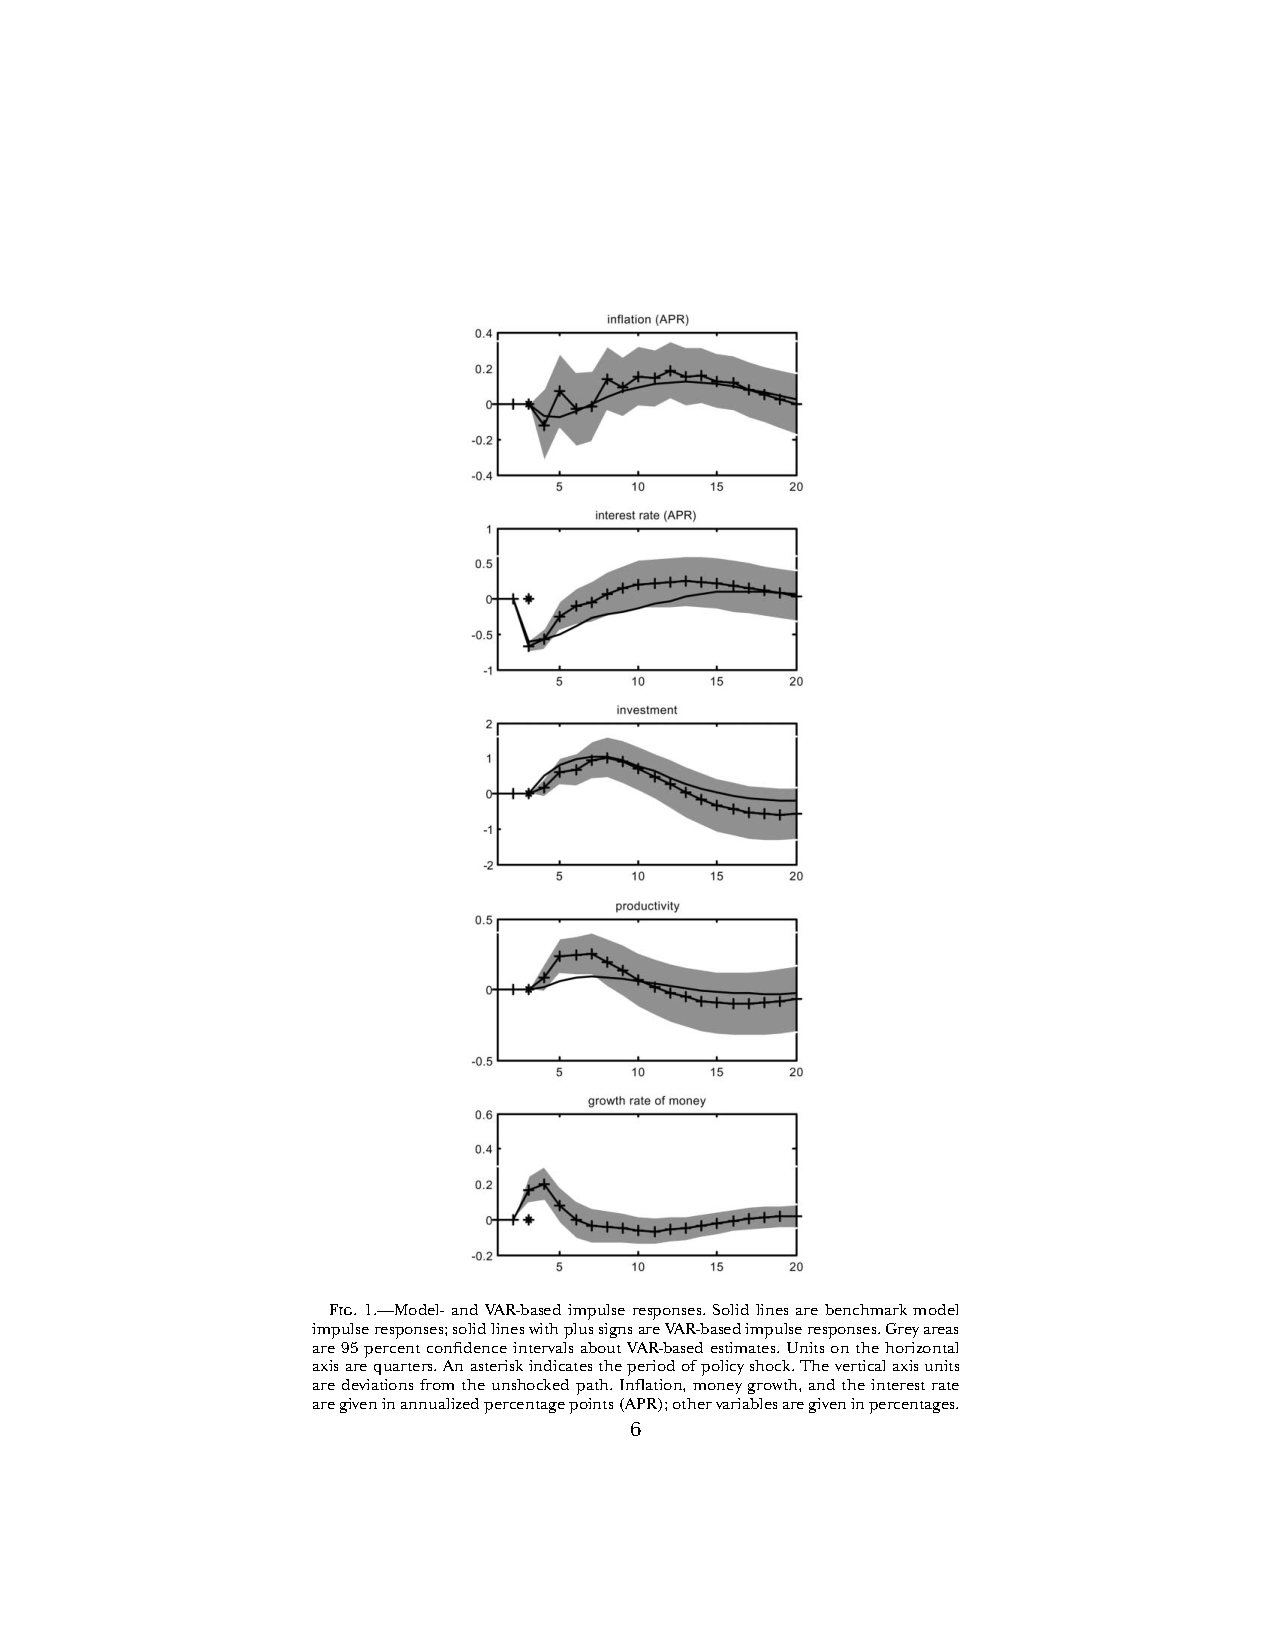
\includepdf[pages=1-]{plots/cev2005.pdf}
\begin{transitionframe}
	\centering { \Huge Restrições de longo prazo}
\end{transitionframe}
\begin{frame}{Restrições na FRI}
	\begin{itemize}
		\item As restrições impostas na seção anterior restringem a resposta {\color{red}contemporânea} das variáveis aos choques fundamentais.
		\item Denotando por $\boldsymbol{F}_h$ a matriz $d \times d$ cuja entrada $(i,j)$ corresponde à resposta da variável $i$ em $t+h$ a um choque em $j$ no período $t$, temos que as restrições de curto prazo focam no comportamento de $\boldsymbol{F}_0$.
		\item Em diversos casos, no entanto, restrições em $\boldsymbol{F}_0$ são difíceis de serem justificadas com base na teoria econômica.
		\item Uma alternativa é {\color{red}considerar restrições na resposta de longo prazo das variáveis aos choques}.
	\end{itemize}
\end{frame}
\begin{frame}{Restrições de longo prazo}
\begin{itemize}
	\item Note que, num SVAR(p) estacionário, inovações em $t$ têm por construção efeito nulo no longo prazo sobre o sistema.
	\begin{itemize}
		\item Do contrário, processo apresentaria raiz unitária.
	\end{itemize}
	\item Isso significa que $\lim_{h \to \infty} \boldsymbol{F}_h = \boldsymbol{0}$, qualquer que seja o valor de $\boldsymbol{B}$ $\implies$ não há restrições para se explorar no comportamento de longo prazo  de $\boldsymbol{F}_h$ que auxiliem na identificação.
	\item Note, no entanto, que, se o SVAR(p) contém uma ou mais variáveis em {\color{blue}primeira diferença}, faz sentido olhar par a {\color{blue}FRI acumulada}, que captura o efeito de choques sobre {\color{blue}o nível das séries diferenciadas}.
		\item FRI acumulada é dada por:
		$$\boldsymbol{G}_h = \sum_{\tau = 0}^h \boldsymbol{F}_\tau$$
\item Possível mostrar que, num SVAR(p) estacionário, FRI acumulada de longo prazo é dada por:
$$\boldsymbol{G}_\infty = \lim_{h \to \infty}\boldsymbol{G}_h = (\mathbb{I} - \boldsymbol{C}_1 - \boldsymbol{C}_2 \ldots - \boldsymbol{C}_p)^{-1} \boldsymbol{B}$$
\end{itemize}
\end{frame}

\begin{frame}{Identificação longo prazo}
	\begin{itemize}
	\item Note que, da expressão de $\boldsymbol{G}_\infty$, se impusermos $d(d-1)/2$ restrições sobre $\boldsymbol{G}_\infty$, obtemos indiretamente  $d(d-1)/2$ restrições sobre $\boldsymbol{B}$.
	\begin{itemize}
		\item Ideia da identificação de longo prazo é gerar restrições sobre $\boldsymbol{B}$ indiretamente via $\boldsymbol{G}_\infty$ que sejam mais palatáveis economicamente.
	\end{itemize}

			\item \textbf{Exemplo:} \citet{blanchard1989dynamic} consideram o seguinte SVAR(p) \textit{trend-stationary} para a economia americana, de 1950-T2 a 1987-T4:
			
			$$\begin{bmatrix}
				\Delta \log(\text{PIB})_t \\
				\text{tx\_desemprego}_t  			\end{bmatrix} = \boldsymbol{c}_0 +\boldsymbol{c}_1 t + \sum_{j=1}^8\boldsymbol{C}_j \begin{bmatrix}
				\Delta \log(\text{PIB})_{t-j} \\
				\text{tx\_desemprego}_{t-j} 			\end{bmatrix}  + \boldsymbol{B} \begin{bmatrix}
					\epsilon^d_t \\
					\epsilon^s_t
				\end{bmatrix}
$$
	onde $\epsilon^s_t$ e $\epsilon^d_t$ são os choques fundamentais do lado da oferta e da demanda na economia. 
	\item {\color{red}Hipótese de identificação:} choques de demanda não exercem efeito de longo prazo sobre a atividade econômica (neutralidade da demanda agregada no longo prazo). Essa hipótese implica que:
	$$\boldsymbol{G}_\infty  = \begin{bmatrix}
	{\color{red}0} & g_{1,2}\\
		g_{2,1} & g_{2,2}
	\end{bmatrix}$$
\end{itemize}
\end{frame}


\begin{frame}{\citet{blanchard1989dynamic} : resultados}
\centering 
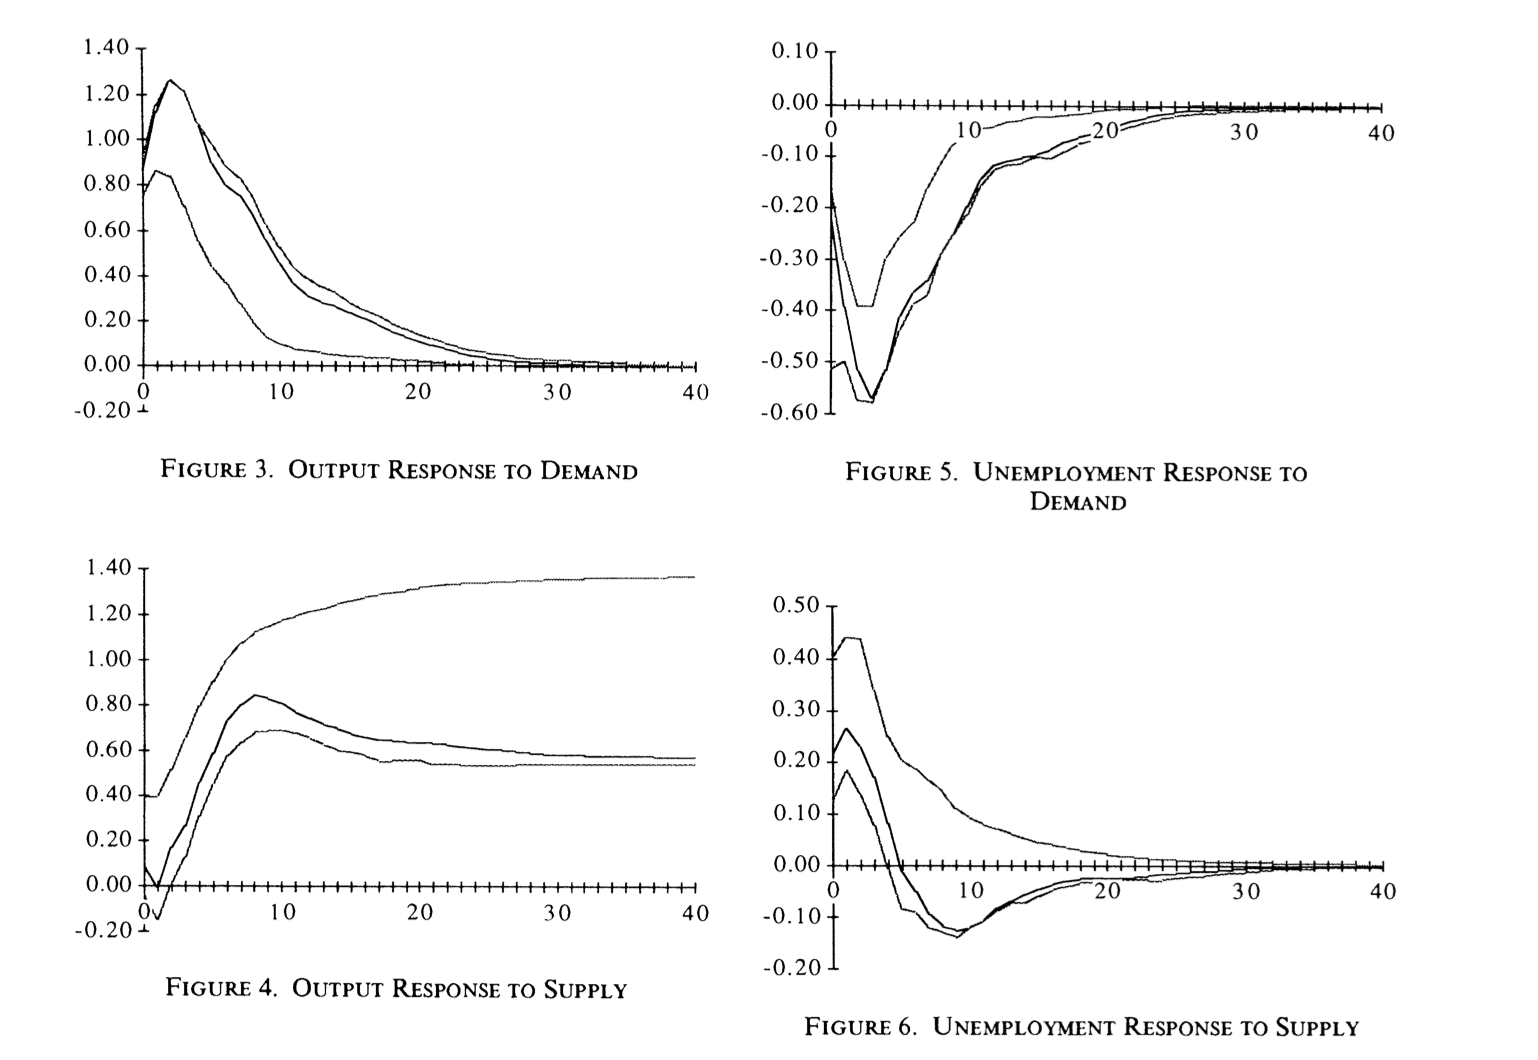
\includegraphics[scale=0.4]{plots/blanchard_quah.png}
\end{frame}

\begin{transitionframe}
	\centering
	{\Huge Restrições de sinal}
\end{transitionframe}

\begin{frame}{Restrições menos estringentes}
\begin{itemize}
	\item As restrições utilizadas anteriormente são bastante fortes, uma vez que pedem que alguma resposta seja exatamente \textbf{zero}.
	\item Restrições mais palatáveis podem ser obtidas trabalhando-se com {\color{blue}restrições de sinal}, em que impomos que as FRI $\boldsymbol{F}_h$ em diferentes horizontes devem ter (alguns) sinais tais quais os prescritos pela teoria.
\begin{itemize}
	\item Por exemplo, a resposta da $i$-ésima variável ao $j$-ésimo choque no horizonte $h$ deve ser não negativa, isto é $F_h(i|j)\geq 0$.
	\item Como a matriz $\boldsymbol{F}_h$ depende de $\boldsymbol{B}$, colocamentos indiretamente restrições sobre estes coeficientes.
\end{itemize}
		\item Dada a natureza mais fraca dessas hipóteses, elas não necessariamente garantem identificação completa do sistema (e, mesmo que garantissem, a verificação de que isso de fato seria o caso é bastante complicada) $\implies$ métodos Bayesianos são preferíveis nesse caso.


	

\end{itemize}
\end{frame}

\begin{frame}{Exemplo}
	\begin{aquote}{\citeauthor{antolin2018}}
	SVARs identified using zero restrictions have consistently found that an exogenous increase in the fed funds rate induces a reduction in real activity. This intuitive result has become the “consensus.” This consensus view, however, has been challenged by Uhlig (2005), who criticizes imposing a questionable zero restriction on the IRF of output to a monetary policy shock on impact. To solve the problem he proposes to identify a shock to monetary policy by imposing sign restrictions only on the IRFs of prices and non-borrowed reserves to this shock, while imposing no restrictions on the IRF of output. The lack of restrictions on the IRF of output to a monetary policy shock makes this is an attractive approach.
\end{aquote}
\end{frame}

\begin{frame}{\citet{uhlig2005}}
\begin{itemize}
	\item \citet{uhlig2005}: VAR(12), sem componentes determinísticos, com dados mensais de janeiro de 1965 a dezembro de 2003. 
	\item Seis variáveis no sistema: PIB real (interpolado), deflator do PIB, índice de preços de commodities, reservas totais, reservas próprias e taxa de juros. Todas em $\log$ e em nível, a não ser juros que é usado diretamente em nível.
	\item Restrições de sinal: FRIs do deflator do PIB, índice de preços de commodities e reservas próprias a um choque monetário contracionista são menores ou iguais a zero, nos horizontes 0 a 5.  FRIs da taxa de juros a um choque monetário contracionista são não negativas, nos horizontes 0 (normalização) e dos horizontes 1 a 5 (política monetária não ``compensa'' plenamente choque monetário contracionista em $t$ nos cinco primeiros meses).
\end{itemize}
\end{frame}

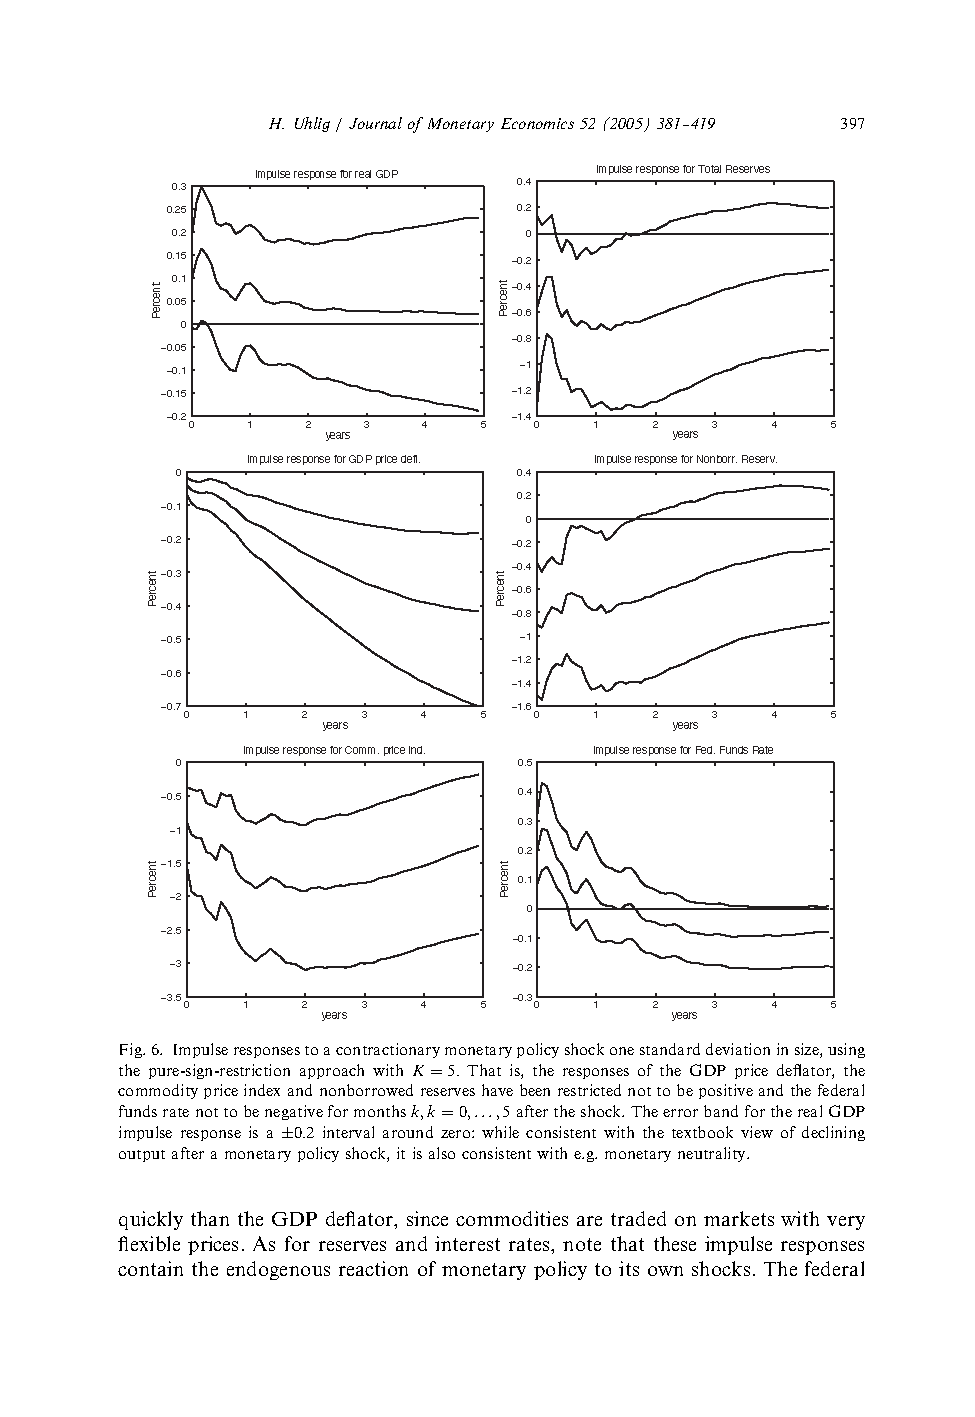
\includepdf[pages=1-]{plots/uhlig.pdf}

\begin{transitionframe}
	\centering
	{\Huge Restrições narrativas}
\end{transitionframe}

\begin{frame}{Usando episódios históricos na identificação}
\begin{itemize}
	\item \citet{antolin2018} sugerem um complemento a restrições de sinal, como forma de fortalecer a identificação.
	\item Ideia é suplementar as restrições de sinais com {\color{blue}restrições narrativas}, derivadas do nosso conhecimento externo de episódios históricos.
	\item Dois tipos de restrições:
	\begin{enumerate}
		\item Restrições nos \emph{sinais} dos choques estruturais: em determinados período de tempo, sabemos que alguns dos choques fundamentais tomaram determinados sinais (surpresas positivas ou negativas).
		\item Restrições sobre a \emph{decomposição histórica} do erro de predição: seja $\boldsymbol{e}_{i,t+h|t} = Y_{i,t+h}-Y_{i,t+h|t}$ o erro de predição que se cometeria em projetar a variável $i$ em $t+h$ com base no SVAR(p) e dados até $t$. 
		\begin{itemize}
			\item 		Pelo que vimos anteriormente, este erro captura a mudança não antecipada (com informação até $t$) da variável $i$, entre $t$ e $t+h$.
			\item Ideia é impor restrições sobre a contribuição dos choques nessa mudança não antecipada: por exemplo, $j$-ésimo choque foi a principal inovação a contribuir para mudança em $i$ na janela.
		\end{itemize}
	\end{enumerate}
			\item As restrições não necessariamente garantem identificação completa $\implies$ métodos Bayesianos são ideais.
\end{itemize}
\end{frame}
\begin{frame}{Exemplo}
	\begin{itemize}
		\item \citet{antolin2018} retornam à análise de \citet{uhlig2005} e suplementam suas restrições de sinal com duas restrições narrativas, com base na mudança na condução da política monetária norte-americana adotada por Paul Volcker em Outubro de 1979:
		
		\vspace{0.5em}
		\begin{quote}
			\footnotesize
			For this reason, in this section we will use narrative sign restrictions for a sin- gle event: October 1979. The monetary policy decisions of October 6, 1979, enacted shortly after Paul Volcker became chairman of the Fed, are described by Romer and Romer (1989) as “a major anti-inflationary shock to monetary policy” and repre- sent, in our view, the clearest case in the postwar period of an exogenous monetary policy shock. Lindsey, Orphanides, and Rasche (2013) provide a detailed account of the events leading to the decision to abandon targeting the federal funds rate in favor of targeting non-borrowed reserves as the operating procedure for controlling the money supply. While macroeconomic conditions, in particular, the deterioration of the inflation outlook and the increase in the real price of oil that followed the Iranian Revolution of 1978–1979, played a large role in causing the shift, the forcefulness and the surprise character of the action and the dramatic break with established practice in the conduct of policy strongly {\color{red}suggest the occurrence of a monetary policy shock}.
		\end{quote}
	\end{itemize}
\end{frame}

\begin{frame}{Choque monetário vs mudança de regime}
	\begin{aquote}{\citeauthor{antolin2018}}
			An argument could be made that the Volcker event is so large that it may be best modeled as a change in the monetary policy rule rather than a monetary policy shock. But Sims and Zha (2006) contend that the evidence for changes in the parameters of the monetary policy rule during the Volcker period is weak and that this period is best described as a period of high variance in the monetary policy shocks to an otherwise unchanged monetary policy rule. Primiceri (2005) reaches similar conclusions. Indeed, as Lindsey, Orphanides, and Rasche (2013) describe, contemporaneous observers accused the FOMC of adopting the new operating procedures only as a smokescreen to obscure its intention to markedly increase short- term interest rates. {\color{red}We side with this view and regard the episode as a large shock within a stable monetary rule}.
	\end{aquote}
	
\end{frame}

\begin{frame}{Restrições utilizadas}
	\begin{itemize}
		\item \citet{antolin2018} valem-se de duas restrições narrativas:
		
		\vspace{1em}
		
		\begin{quote}
			
			\textbf{Narrative Sign Restriction 4 [1]:} The monetary policy shock for the observation corresponding to October 1979 must be of positive value.
			
			
		\textbf{Narrative Sign Restriction 5 [2]: }For the observation corresponding to October 1979, a monetary policy shock is the overwhelming driver of the unexpected move- ment in the federal funds rate. In other words, the absolute value of the contribution of monetary policy shocks to the unexpected movement in the federal funds rate is larger than the sum of the absolute value of the contributions of all other structural shocks.
		\end{quote}
		
	\end{itemize}
\end{frame}

\begin{frame}{Resultados}
\centering 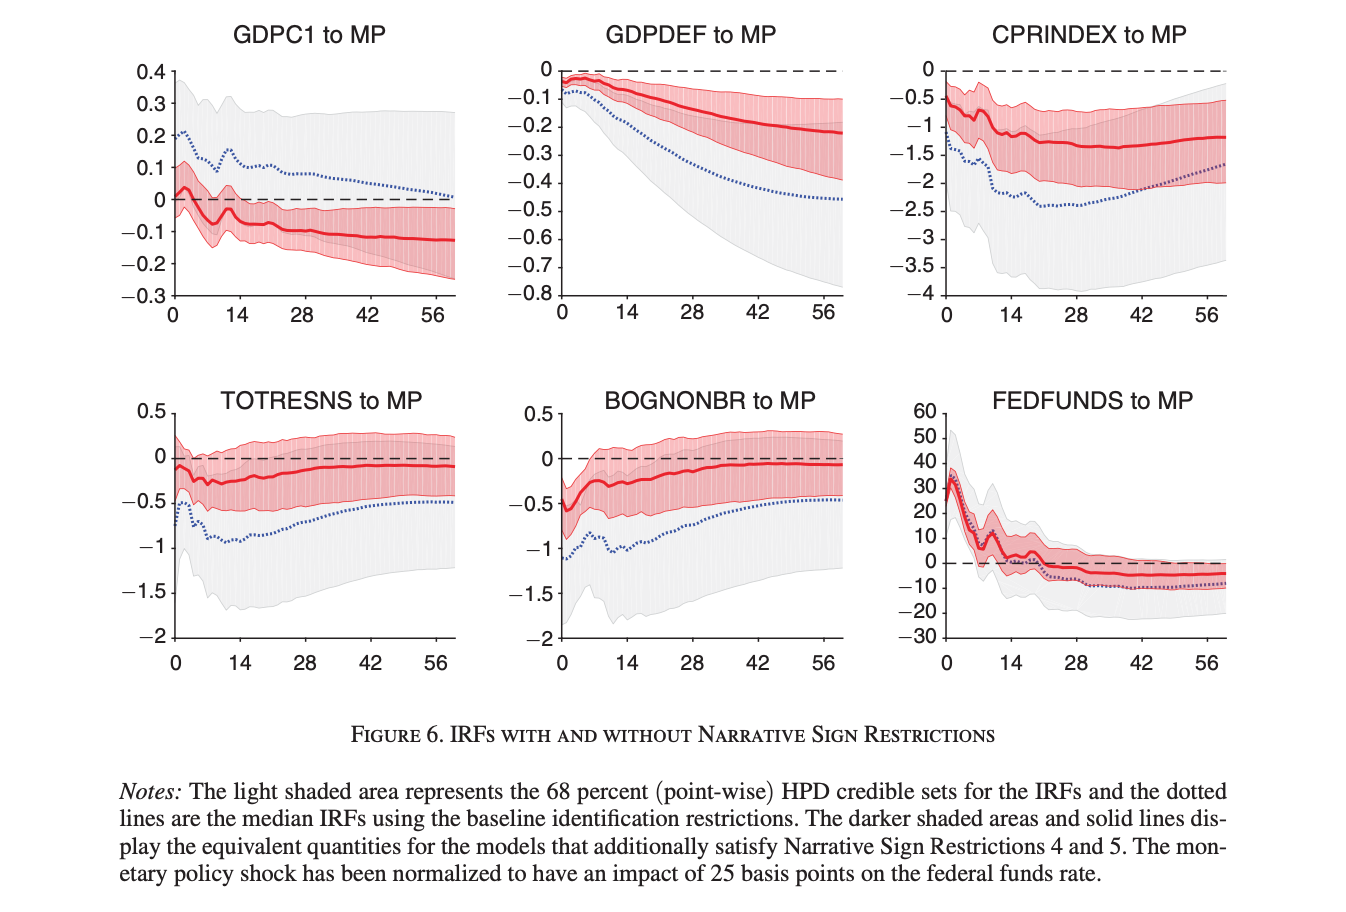
\includegraphics[scale=0.5]{plots/antonil.png}
\end{frame}


\begin{transitionframe}
	\centering { \Huge Identificação por instrumentos externos}
\end{transitionframe}

\begin{frame}{Uma \textit{proxy} para o choque}
	\begin{itemize}
		\item A abordagem de identificação de um SVAR através de instrumentos externos nos permite identificar a {\color{blue}FRI a um dos choques}, sob a hipótese de que observamos uma {\color{blue}boa \textit{proxy} para ele}. 
		\item Uma boa \textit{proxy} para o choque $\epsilon_{jt}$ é uma série de tempo $\{Z_t\}_t$, com as seguintes propriedade:
		\begin{enumerate}
			\item 	(Relevância)	$\operatorname{cor}(Z_t, \epsilon_{jt}) = \rho \neq 0$.
			\item (Exclusão) $\operatorname{cor}(Z_t, \epsilon_{it})  = 0, \quad \forall i \neq j$.
		\end{enumerate}
	\item Instrumento externo é uma boa \textit{proxy} para a inovação fundamental se a prediz, mas não exibe associação com as demais inovações fundamentais.
	\item Sob as duas hipóteses anteriores, e a normalização $b_{jj} = 1$, temos que as respostas contemporâneas de cada variável $i$ do sistema ao choque $j$ são identificáveis como:
	$$F_{0}(i|j) = b_{ij} = \frac{\operatorname{cov}(u_{i,t}, Z_{t})}{\operatorname{cov}(u_{j,t}, Z_{t})} $$
	\end{itemize}
\end{frame}

\begin{frame}{Estimação com instrumento externo}
	\begin{itemize}
		\item O resultado anterior sugere o seguinte procedimento para estimar as FRI a um choque $j$ sob a presença de um instrumento externo.
		\begin{enumerate}
			\item Estimar um VAR(p) reduzido, e guardar seus resíduos $\hat{\boldsymbol{u}}_t$.
			\item Estimar a resposta contemporânea dos choques como $\hat b_{ij}$, onde  o $\hat b_{ij}$ é o estimador de variável instrumental do efeito de $\hat u_{j,t}$ sobre $\hat u_{i,t}$, usando $Z_t$ como instrumento.
			\item Usando o estimador da resposta contemporânea e a propagação dos choques estimada pelo VAR(p), calcular recursivamente a FRI.
		\end{enumerate}
		\item Inferência estatística (quantificação da incerteza) para esse estimador não é imediata.
		\begin{itemize}
			\item \citet{Stock2018} proveem métodos para se levar em conta a incerteza estatística das duas etapas de estimação no cálculo de erros-padrão.
		\end{itemize}		
	\end{itemize}
\end{frame}

\begin{frame}{Instrumento interno}
\begin{itemize}
		\item Se pudermos fortalecer a hipótese de identificação do instrumento para:
	$$\operatorname{cov}(Z_t, \epsilon_{is}|Z_{t-1},\boldsymbol{Y}_{t-1}, Z_{t-2},\boldsymbol{Y}_{t-2},\ldots)  \neq 0 \iff  i =j \text{ e } s = t$$
	então as FRI ao choque $i$ podem ser estimadas incluindo-se $Z_t$ como a {\color{blue}primeira variável} em um VAR(p) reduzido com $\boldsymbol{Y}_t$; calculando, por Choleski, FRI {\color{blue}preliminares} de cada variável a um choque no instrumento, $\tilde{F}_{h}(i|Z)$, e estimando a resposta de $i$ ao choque $j$ em $h$ como:
	$$\hat F_{h}(i|j) = \frac{\tilde{F}_{h}(i|Z)}{\tilde{F}_{0}(j|Z)}  $$
	\item Abordagem de {\color{blue}instrumento interno}.
	\begin{itemize}
		\item Quantificação de incerteza é mais simples.
		\item Metodologia é robusta a problemas de {\color{blue}invertibilidade}, i.e. se modelo estrutural completo que temos na cabeça envolve mais variáveis do que as efetivamente incluídas no SVAR \citep{plagborg2021}.
	\end{itemize}
\end{itemize}
\end{frame}

\begin{frame}{Instrumentos externos para política monetária}
	\begin{itemize}
		\item  Literatura consolidada em macroeconometria visa a estimar os efeitos de surpresas não antecipadas na política monetária através de construção de mensurações diretas do que seria a surpresa.
		\begin{itemize}
			\item \citet{Romer2004}: série de surpresa monetária a partir das atas internas do Federal Reserve americano e sua meta de taxa de juros, implícita ou explícita, nas discussões ({\color{blue}\textit{instrumento narrativo}}). 
			\begin{itemize}
				\item Para separar o que é surpresa do sistemático, utiliza-se o resíduo de uma regressão da variação da meta taxa de juros (série narrativa) na variação das projeções internas do Fed, de modo a capturar o componente surpresa (não sistemático) da política.
			\end{itemize}
						\item \citet{Gertler2015}: série de surpresa monetária é calculada a partir da variação, em alta frequência, das curvas de juros futuras no mercado financeiro, em torno da janela de anúncio da política monetária americana ({\color{blue}\textit{instrumento de alta frequência}}).
						\begin{itemize}
							\item Sob não arbitragem e uma janela de curta duração, variação é atribuível ao componente não antecipado da política monetária.
						\end{itemize}
		\end{itemize}
	\end{itemize}
\end{frame}

\begin{frame}{Separando surpresa monetária de choques informacionais}
	\begin{wideitemize}
		\item \citet{Miranda2021} apresentam algumas críticas aos instrumentos externos usados na literatura.
		\begin{itemize}
			\item Instrumento narrativo de \citet{Romer2004} é serialmente autocorrelacionado e sistematicamente associado com mudanças antecipadas de política monetária (\textit{forward guidance}), o que indica que ele não é uma boa proxy para a surpresa monetária.
			\item Instrumento de alta frequência de  \citet{Gertler2015} é predizível com base nas projeções internas do Fed, o que sugere que anúncios de política monetária contém um {\color{blue}componente informacional}, para além do choque monetária
		\end{itemize} 
			\item Para capturar o choque monetário, separando-o da informação acerca da economia divulgada pelo Fed, \citet{Miranda2021} trabalham com o resíduo da série de \citet{Gertler2015} numa regressão das projeções internas do Fed.
	\end{wideitemize}
	\end{frame}
	
	\begin{frame}{Resultados}
		\centering
		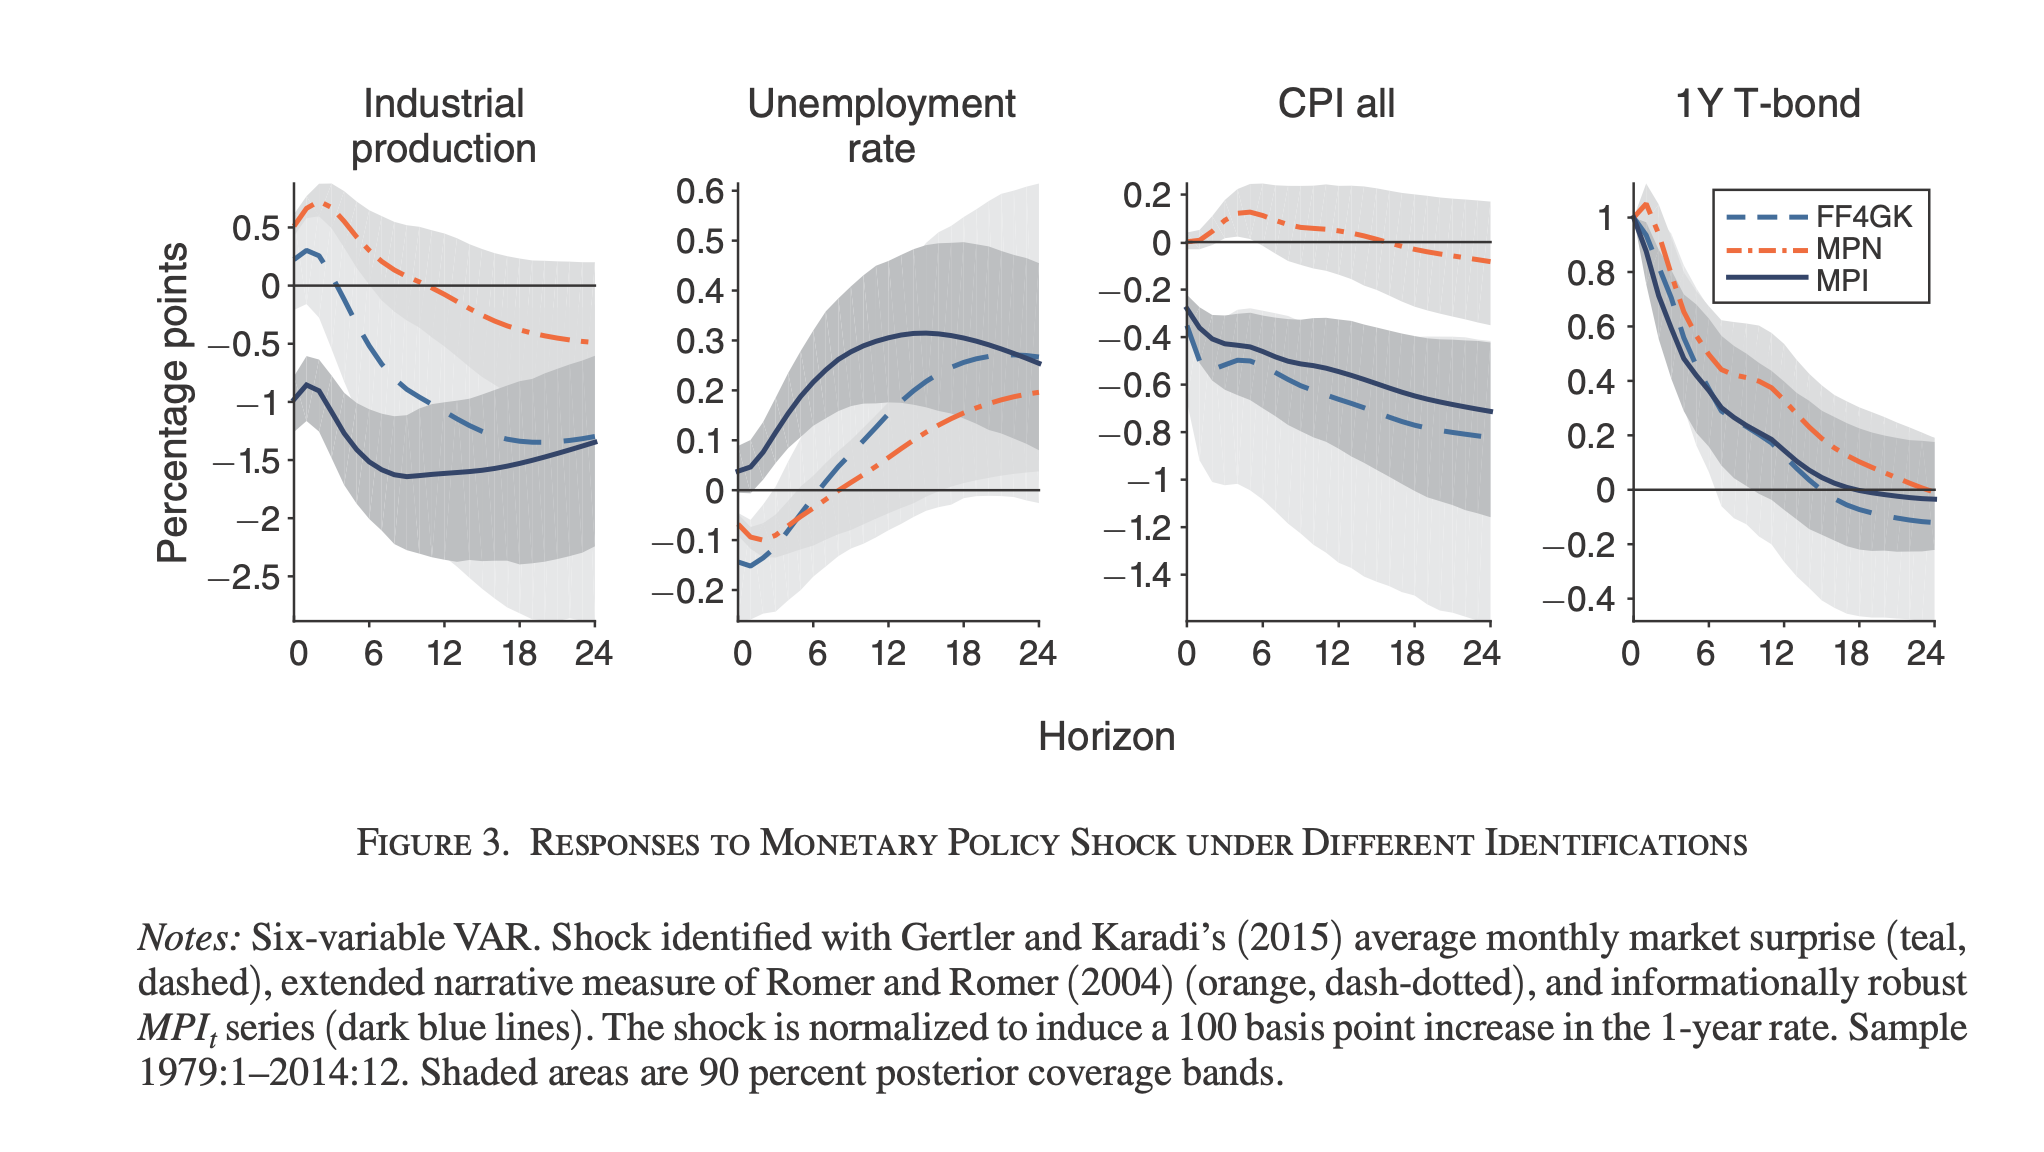
\includegraphics[scale=0.3]{plots/miranda.png}
	\end{frame}

\begin{transitionframe}
	\centering { \Huge Identificação por heterocedasticidade}
\end{transitionframe}

\begin{frame}{Ideia de identificação por heterocedasticidade}
	\begin{itemize}
		\item A ideia desta estratégia de identificação consiste em argumentar que existem regimes na economia em que a volatilidade relativa dos choques muda, mas que os parâmetros estruturais correspondentes à resposta aos choques permanecem os mesmos.
		\begin{itemize}
		\item Sob essa hipótese, é possível usar a variação na volatilidade como ``instrumento'' para recuperar as respostas aos choques.
	\end{itemize}
		\item Como exemplo, suponha que temos um SVAR(p) bivariado.
		\item Nesse caso, sob a normalização de que $b_{i,i} = 1$, o problema de identificação consiste em recuperar $b_{1,2}$ e $b_{2,1}$, separando-os da variância dos choques estruturais.
		\begin{itemize}
			\item A princípio, temos quatro parâmetros e somente três equações dadas por $\mathbb{V}[\boldsymbol{u}_t]$, i.e. falta uma restrição.
		\end{itemize}
	\end{itemize}
\end{frame}
\begin{frame}{Mudança de regime e identificação}
	\begin{itemize}
		\item Suponha que existe um período de tempo $T^*$, que {\color{blue}define uma mudança de regime}.
		\begin{itemize}
				\item No regime $t < T^*$, os choques fundamentais tem variância $\sigma_{1}^2(1)$ e $\sigma_{2}^2(1)$.
		\item No regime $t \geq T^*$, os choques fundamentais têm variância $\sigma_{1}^2(2)$ e $\sigma_{2}^2(2)$.
		\end{itemize}
		\item Sob a hipótese de que $b_{1,2}$ e $b_{2,1}$ mantém-se {\color{blue}invariantes} entre os regimes, temos que a matriz de variância-covariância dos erros em forma-reduzida, nos regimes 1 e 2, nos recupera:
		
		$$\mathbb{V}[\boldsymbol{u}_t|t<T^*] = \begin{bmatrix}
			1 & b_{1,2} \\
			b_{2,1} & 1 
		\end{bmatrix} \begin{bmatrix}
		\sigma^2_1(1) & 0  \\ 
		0 & \sigma^2_2(1)
		\end{bmatrix}  \begin{bmatrix}
		1 & b_{2,1} \\
	 b_{1,2}  	& 1 
		\end{bmatrix} $$ 
		
			$$\mathbb{V}[\boldsymbol{u}_t|t\geq T^*] = \begin{bmatrix}
			1 & b_{1,2} \\
			b_{2,1} & 1 
		\end{bmatrix} \begin{bmatrix}
			\sigma^2_1(2) & 0  \\ 
			0 & \sigma^2_2(2)
		\end{bmatrix}  \begin{bmatrix}
			1 & b_{2,1} \\
			b_{1,2}  	& 1 
		\end{bmatrix} $$ 
			\item Sistema com seis parâmetros e seis restrições!
	\end{itemize}

\end{frame}

\begin{frame}{Identificação por heterocedasticidade}
	\begin{itemize}
		\item É possível mostrar que o sistema anterior tem solução única se, e somente se, $\frac{\sigma^2_1(2)}{\sigma^2_1(1)} < \frac{\sigma^2_2(2)}{\sigma^2_2(1)}$ ou $\frac{\sigma^2_1(2)}{\sigma^2_1(1)} > \frac{\sigma^2_2(2)}{\sigma^2_2(1)}$.
		\begin{itemize}
			\item Isto é, se a importância relativa dos choques fundamentais muda entre os regimes.
		\end{itemize}
		\item Num SVAR(p) com mais de duas variáveis, de modo geral, precisamos de mais de duas mudanças de regime para identificar os parâmetros.
		\begin{itemize}
			\item Estimação pode ser feita por máxima verossimilhança condicional, impondo a estrutura de quebra no sistema.
		\end{itemize}
		\item No entanto, no caso particular em que, num SVAR(p) genérico, temos somente uma mudança de regime, {\color{blue}mas sabemos que a variância de \textbf{somente um} dos choques muda entre regimes} (por exemplo, o primeiro), é possível identificar a FRI desse choque, pois, nesse caso:
		$$b_{i,1} = \frac{\operatorname{cov}(u_{i,t}, u_{1,t}|t\geq T^*)- \operatorname{cov}(u_{i,t}, u_{1,t}|t< T^*)}{\mathbb{V}[u_{1,t}|t\geq T^*]-\mathbb{V}[u_{1,t}|t< T^*]}$$
	\end{itemize}
\end{frame}

\begin{frame}{Exemplo}
\begin{itemize}
	\item 	\citet{Wright2012} estuda a transmissão da política monetária sobre os preços de ativos nos Estados Unidos.
	\item VAR(p) com dados diários de seis preços financeiros: títulos públicos de maturidade de dez e dois anos, taxa de inflação anual média \textit{breakeven} no horizonte de cinco anos, taxa de inflação anual média \textit{breakeven} para os cinco anos após os próximos dez anos, taxas de juros de dívidas corporativa de nota BAA e AAA. Janela de novembro de 2008 a setembro de 2011.
	\begin{itemize}
		\item Ideia é entender transmissão de política monetária num regime de juro de curto prazo zero.
	\end{itemize}
	\item Estratégia de identificação: nos dias de anúncio de política monetária, a variância dos choque monetário é maior do que nos dias sem anúncio, e a variância dos demais choques estruturais mantém-se constante.
	\begin{itemize}
		\item Dois regimes intermitentes no tempo, mas argumento de identificação é idêntico ao discutido anteriormente.
	\end{itemize} 
\end{itemize}
\end{frame}

\begin{frame}{Resultados}
\centering
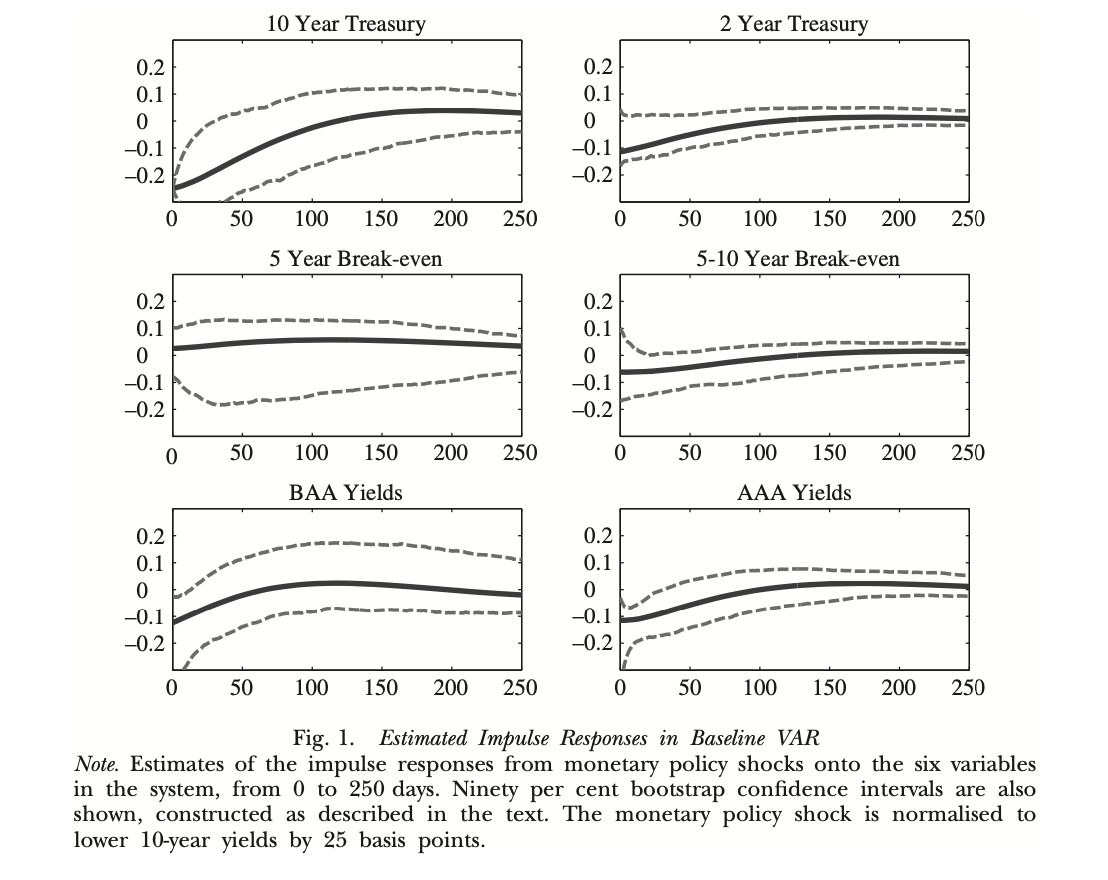
\includegraphics[scale=0.5]{plots/wright.png}
\end{frame}

\appendix
\begin{frame}[allowframebreaks]{Referências}
	\printbibliography
\end{frame}
\end{document}

